\documentclass[12pt]{report}
\usepackage[utf8]{inputenc}
\usepackage{graphicx}
\usepackage{hyperref}
\usepackage{hyperref}
\hypersetup{
    colorlinks=true,
    linkcolor=blue,
    filecolor=magenta,      
    urlcolor=cyan,
}
\usepackage{url}
\usepackage{geometry}
 \geometry{
 a4paper,
 total={170mm,257mm},
 left=20mm,
 top=20mm,
 }
% \title{Seminar Report \\ on \\ Guaranteed Real-Time Control Methodologies Using Open-Source Tools}

% \author{Sudhakar Kumar \\ 183236001 \\ Department of Systems and Control Engineering \\ IIT Bombay}
% \date{\today}

\begin{document}

% \maketitle


\begin{titlepage}
	\centering
	
\includegraphics[width=0.4\textwidth]{images/iitb1.png}\par\vspace{1cm}
	{\scshape\LARGE IIT Bombay \par}
	\vspace{1cm}
	{\scshape\Large Seminar Report\par}
	\vspace{0.5cm}
	{\Large on \par}
	\vspace{0.5cm}
	{\huge\bfseries Real-Time Control Methodologies Using Open-Source Tools\par}
	\vspace{0.5cm}
	{\Large by \par}
	\vspace{0.5cm}
	{\Large Sudhakar Kumar \\ Roll No. 183236001 \par}
	\vfill
	\large{Under the supervision of}\par
	\Large{Prof. Kannan Moudgalya \\ Department of Chemical Engineering \\ Indian Institute of Technology Bombay \\ Mumbai 400 076, INDIA}

	\vfill

% Bottom of the page
	{\large \today\par}
\end{titlepage}
\tableofcontents
\listoffigures
%\listoftables

\chapter{Introduction}
Commercial usage of computers started off somewhat around in 1951 when UNIVAC (stands for Universal Automatic Computer) was dedicated by the U.S. Census Bureau. By analyzing the timeline of computers' evolution, we can superficially divide this period (i.e. 1951-present) into three generations of computing namely mainframe, personal computers (better known as PC), and post-PC. The mainframe computer was marked by expensive computers that were too expensive to be afforded by individuals, and each computer served a large number of users. Even today, mainframe computers are treated as data servers that are capable of processing large-scale transactions and thus, these are primarily used by large organizations for critical applications. Though the mainframe computers always outperformed PC, it was the PC era which witnessed the revolutionary emergence of desktops. Unlike mainframe computers, the PCs have proved to be cost-effective which could be afforded by the individual users. %\cite{framevspc}. 
The post-PC era is a witness of the emergence of small and portable computers along with the computers embedded in everyday applications. In this post-PC era, an individual is interacting with several computers (or mini-computers) in his/her day-to-day activities  \cite{NPTEL}. Most of these computers, which individuals are interacting with, fall under the umbrella of embedded real-time systems (ERTS). \\

An embedded system is nothing but a computer system. However, unlike general PCs, an embedded system has a dedicated function within a large (mechanical or electrical) system. In the first two computing generations (mainframe and PC), real-time and embedded computing applications were confined to only a handful applications in space and defense sectors. Nonetheless, the post-PC era of computing noted a surge in the usage of ERTS, which has already touched every facet of our life. The previous statement can be corroborated by the fact that several gadgets and applications, which have today become indispensable to our everyday life, are actually ERTS (in some form or the other). For example, we have pervasive consumer products such as digital cameras and cell phones; telecommunication domain products such as set-top boxes and video conferencing applications; office products such as fax machines, laser printers, and security systems. Besides, we encounter ERTS in hospitals as well. These could be in the form of medical instrumentation equipment and imaging systems. \\

Some of the reasons which can be attributed to the phenomenal proliferation of ERTS in day-to-day life are reductions in the size and the cost of the computers, combined with the improvements to their performance. The availability of computers at rapidly falling prices, reduced weight, rapidly shrinking sizes, and their increasing processing power have together contributed to the present scenario. The rapid growth of applications deploying real-time technologies has been matched by the evolutionary growth of the underlying technologies supporting the development of real-time systems. Hence, we strongly believe that there is a need to study the tools which facilitate real-time sensing and control systems. Adding to this, we need to focus on the open-source tools which would reduce our dependency on proprietary solutions and help us create cost-effective solutions for the entire society. In this report, we will discuss some of the technologies utilized in developing real-time systems, with restricting this discussion to the open-source tools which (can) guarantee the real-time control methodologies. The rest of the report is organized as follows. \\ 

In the second chapter on Real-Time Systems, we will define the concept of real-time and its comparison with respect to logical time. For a real-time system, if an answer i.e. the system's response to externally generated input stimuli is late, it's wrong. We will investigate the timing constraints for a real-time system along with its applications in industry, defense, aerospace, etc. Subsequently, a basic model, along with its important functional blocks, of a real-time system is presented. Next, we discuss the key characteristics of real-time systems, which must be met while dealing with these systems. At the end of this chapter, we explain the hard real-time tasks, firm real-time tasks, and soft real-time tasks. \\ 

In the third chapter on Real-Time Task Scheduling, we will discuss the available scheduling algorithms for real-time tasks. The two main types of schedulers are: clock-driven and event-driven. Along with these two types, we discuss their sub-types briefly. We will have a look at the comparison between clock-driven scheduling and event-driven scheduling. Along with these two traditional scheduling algorithms, we will explain dynamic scheduling, in which the hardware determines which instructions to execute, as opposed to a statically scheduled machine. Subsequently, we will discuss two important dynamic scheduling algorithms which have been immensely useful in real-time sensing and control systems. \\ 

In the fourth chapter on Real-Time Operating Systems (RTOS), we examine the important features that an RTOS is expected to support. Here, we discuss the key features which are quintessential for an RTOS and are usually missing in a General Purpose Operating System (GPOS). Along with this, we elaborate the concept of multitasking and context switching. Next, we investigate whether Unix or Windows qualify for an RTOS.  The  traditional  Unix  operating  system suffers  from  several  shortcomings  when  used  in  real-time  applications. Windows NT has several features which are very desirable for real-time applications such as support for multi-threading, real-time priority levels, and timer. However, it is neither advisable nor feasible to use NT for hard real-time applications, for example, at the controller level with sub-millisecond precision. At the end of this chapter, we summarize the major differences between a GPOS and an RTOS. \\

In the fifth chapter on Tools for enabling Real-Time Features, we explain the open-source tools which are being utilized to enable real-time constraints across various platforms like an operating system, open-source software like Scilab, OpenModelica, and micro-controllers like Arduino. For enabling Linux as a real-time system, we describe three important patches/extensions namely, PREEMPT\_RT, RTLinux, and RTAI. With RTAI-Lab and Scilab,  it is possible to obtain a complete open source environment for designing control systems and test them in real physical systems.  This software tool-chain is equivalent to the proprietary software for control systems Labview or Dspace. Next, we will discuss the tools available in OpenModelica – Modelica.\texttt{StateGraph} and Real-Time simulation flag – which can be used to characterize reactive systems and the physical time concept of real-time systems. Next, we create a task of blinking two LEDs at different rates using FreeRTOS on Arduino Uno. Finally, we present a discussion on when and where we should use FreeRTOS. At the end, we conclude our report with the subtleties of a real-time system along with the performance of open-source tools for enabling real-time features on various platforms. 
 
 \chapter{About Real-Time Systems}
Real-time is a quantitative notion of time i.e., it is measured using a physical (real) clock. Whenever we quantify time using a physical clock, we deal with real-time. For example, we will consider an automated chemical plant. In this plant, the moment the temperature of the reaction chamber reaches a certain pre-specified temperature, the system automatically switches off the heater within a pre-determined time interval, say within 30 milliseconds. While describing this behavior of the chemical plant, the referred time value signifies the readings of some physical clock existing in the plant automation system.\\ 

Unlike real-time, logical time deals with a qualitative notion of time and is manifested by event ordering relations. Hence, time readings from a physical clock are not required for ordering the events while dealing with logical time. For example, we will review the behavior of library automation software: ``After a user enters a command to query for a book, the details of all matching books are displayed." In this example, the events  ``query book command" and ``display of results" are logically ordered in terms of the sequence of the events. Here, we don't notice any quantitative expression of time. Thus, this behavior of library automation software is devoid of any real-time considerations.

\begin{figure}[h]
    \centering
    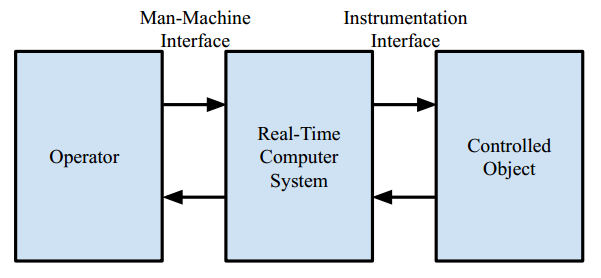
\includegraphics[width=0.6\textwidth]{images/real-time-sys.png}
    \caption{Real-Time Systems}
    \label{fig:rts}
\end{figure}

We will revisit the example of an automated chemical plant to study other features of a real-time system (RTS). Suppose that the controlling computer system of the chemical reaction in the plant stated above has stopped functioning. What would happen to the chemical reaction then? Will it stop or keep changing its state? Undoubtedly, the reaction will continue to change its state. Thus, we can note that an RTS changes its state as a function of physical time \cite{rts}. Based on this assumption, one can decompose an RTS into a set of subsystems, as shown in figure \ref{fig:rts}. A real-time computer system must react to stimuli from the controlled object (or the operator) within time intervals dictated by its environment. In other words, an RTS is any information processing system which has to respond to externally generated input stimuli within a finite and specified timing constraint \cite{unsw}. In  these systems, 
\begin{itemize}
  \setlength\itemsep{-0.2em}
    \item Correctness of the system behavior depends not only on the logical results of the computations, but also on the physical instant at which these results are produced. 
    \item Failure to respond in time is as bad as the wrong response! 
\end{itemize}
Thus, the key thing to remember about an RTS is that in an RTS if an answer is late, it's wrong. In this era of technology, all of us use a PC (with different operating systems) every now and then. One can argue that all operating systems are real-time. That is, they all have some kind of deadline. According to  Mr. Steven Rostedt (a Linux kernel developer at Red Hat and maintainer of the stable version of the real-time Linux kernel patch), ``If we hit a key and the computer does not respond in say 5 minutes, we are likely to throw the computer out the window" \cite{rtlinux}. It failed to meet its deadline. When our deadlines are big enough, pretty much any operating system will do. \\

Let us say, we are plotting a series of data using a GPOS running on a PC. Ideally, we should expect our PC to generate the plot in a couple of seconds (like 2-3 seconds). However, we won't mind even if this operation is delayed by one more second as there's no real impact of this delay. On the contrary, consider the event of plotting the series of data vis-\`a-vis applying a brake in a car, where the delay of even one second could be catastrophic. Thus, RTSs are exploited to deal with such events where we cannot afford a delay of even one second. 

\section{Applications of Real-Time Systems}
There are quite a few applications of RTSs in wide ranging areas. In the following subsections, we list some of the prominent areas like industries, defense, aerospace, etc. where RTSs are extensively exploited. 

\subsection{Industrial Applications}
\noindent \textbf{Chemical Plant Control}\\
We will reconsider chemical plant control systems. In an automated chemical plant, a real-time computer is deployed to periodically monitor the plant conditions. These plant conditions are determined by the parameters like current readings of pressure, temperature, chemical concentration of the reaction chamber, etc. Based on the values sampled at a given instant, the automation system decides on the corrective actions which are deemed mandatory at that instant for maintaining the chemical reaction at a certain rate. Each time the plant conditions are sampled, the automation system should not only decide on the exact instantaneous corrective actions required such as changing the pressure, temperature, chemical concentration, etc. but also perform these actions within certain predefined time bounds. Typically, the time bounds in such chemical plant control applications range from a few microseconds to several milliseconds.\\

\noindent\textbf{Supervisory Control and Data Acquisition (SCADA)}\\
A SCADA system is a control system architecture that helps monitor and control a large number of distributed events of interest. In these systems, sensors are dispersed at various geographic locations to collect raw data. These raw data, known as events of interest, are then processed and stored in a real-time database, which reflects the current state of the environment. To ensure that the database presents a pragmatic model of the up-to-date state of the environment, the database is updated frequently. An example of a SCADA system is a system that monitors and controls traffic in a computer network. Depending on the load being discerned in different segments of the network, the SCADA system makes the router change its traffic routing policy in a dynamic fashion. The time constraint in such a SCADA application should make sure that the sensors must sense the system state at regular intervals (say every few milliseconds) and the same must be processed before the next state is sensed.\\


\noindent\textbf{Automated Car Assembly Plant}\\
In these plants, the work product, which is a partially assembled car, moves on a conveyor belt, as shown in figure \ref{fig:car}. As we can observe that several workstations are placed by the side of the conveyor belt. Each workstation is responsible for executing some specific work on the work product such as fitting engine, fitting door, spraying paint, etc. as it moves on the conveyor belt. A chassis is introduced near the first workstation on the conveyor belt and a finished car comes out after the work product goes past all the workstations. At each workstation, a sensor senses the arrival of the next partially assembled product. As soon as the partially assembled product is sensed, the workstation begins to execute its work on the work product. The time constraint imposed on the workstation computer should ensure that the workstation must complete its work before the work product moves on to the next workstation. The time bounds involved here are typically of the order of a few hundreds of milliseconds. 
\begin{figure}[h]
    \centering
    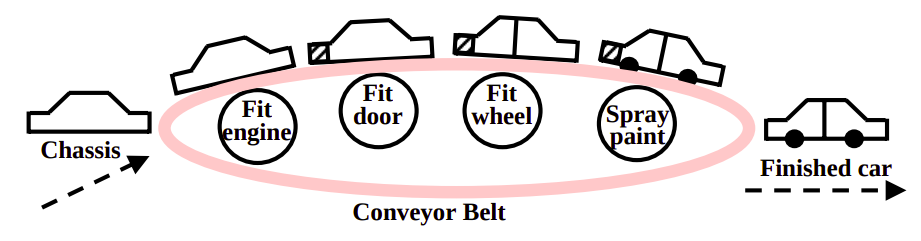
\includegraphics[width=0.8\textwidth]{images/car-assembly.png}
    \caption{Schematic Representation of an Automated Car Assembly Plant }
    \label{fig:car}
\end{figure}



\subsection{Defense Applications}
\noindent\textbf{Missile Guidance System}\\
A guided missile is capable of sensing an intended target and strikes it. Once the target is sensed and detected, the missile needs to follow a trajectory to strike the target with utmost precision. In a missile guidance system, missile guidance is achieved by a computer (mounted on the missile), which computes the deviation from the required trajectory and affects track changes of the missile. The time constraint on the guidance system should ensure that sensing and track correction tasks must be activated frequently enough to maintain the missile's trajectory. The time bounds involved in the tasks of target sensing and track correction are typically within a few hundreds of microseconds or even lesser. In case of missile guidance system, the time bound largely depends upon the speed of the missile and the type of the target. 

\subsection{Aerospace Applications}
\noindent\textbf{Computer On-board an Aircraft}\\
In modern aircrafts, a pilot can opt for ``auto pilot" mode while flying aircraft. As the name indicates, in ``auto pilot" mode, an on-board computer takes over all controls of the aircraft including navigation, take-off, and landing of the aircraft. Subsequently,  the computer periodically samples velocity and acceleration of the aircraft. From the sampled data, the on-board computer computes $X$, $Y$, and $Z$ coordinates of the current aircraft position and compares them with the pre-specified track data. Before the next sample values are obtained, it computes the deviation from the specified track values and takes corrective actions, if needed. In this case, the time bound involved in the tasks of sampling of the various parameters and their processing are typically within a few micro seconds. \\

Now, we summarize the average time bound for all the above mentioned applications, as given in the table \ref{table:1}. It would help us understand the timing requirements for an RTS. 
\begin{table}[h]
\centering
\begin{tabular}{|c|c|}
 \hline
 \textbf{Applications} & \textbf{Time bound} \\
 \hline \hline
 Chemical plant control & few microseconds to several milliseconds \\ 
 \hline
SCADA & few milliseconds \\ 
 \hline
 Automated car assembly plant & few hundreds of milliseconds\\ 
 \hline
 Missile guidance system & few hundreds of microseconds\\ 
 \hline
 Computer on-board an aircraft & few microseconds \\
 \hline
\end{tabular}
\caption{Applications of Real-Time Systems with its Time Bound}
\label{table:1}
\end{table}

From the table \ref{table:1}, we can infer that in case of RTSs, the time bound ranges from a few microseconds to a few milliseconds. 

\section{Basic Model of a Real-Time System}
The figure \ref{fig:model} shows a simple model of an RTS. Here, the sensors are interfaced with the input conditioning unit, which in turn is connected to the input interface. On the other hand, the output interface, output conditioning unit, and the actuator are interfaced in a complementary manner. The figure \ref{fig:model} can be easily related with the figure \ref{fig:rts}. where we decomposed an RTS into a set of subsystems, namely operator, real-time computer system, and controlled object.  Now, we
briefly describe the roles of the different functional blocks given in figure \ref{fig:model}. 
\begin{figure}[h]
    \centering
    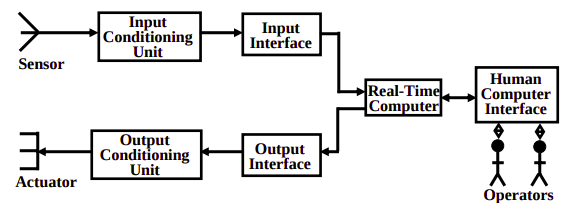
\includegraphics[width=0.8\textwidth]{images/model-rts.png}
    \caption{Model of a Real-Time System}
    \label{fig:model}
\end{figure}

\begin{itemize}
    \item \textbf{Sensor}: A sensor is a device or module whose purpose is to sense the change in its environnment and pass on this information to the connected electronic circuits. Thus,  it converts some physical characteristic of its environment into electrical signals. An example of a sensor is a photo-voltaic cell which converts light energy into electrical energy.
    \item \textbf{Actuator}: An actuator is a device that takes its inputs from the output interface of a computer and converts these electrical signals into some physical actions on its environment. The physical actions may be in the form of motion, change of thermal, electrical, or physical characteristics of the objects. Motor is a popular actuator.
    \item \textbf{Signal Conditioning Units}: The electrical signals produced by a computer can hardly ever be used to directly drive an actuator. The computer signals usually need conditioning before they can be used by the actuator. This is termed as output conditioning. Similarly, input conditioning is required to be performed on sensor signals before they can be accepted by the computer. For example, analog signals generated by a photo-voltaic cell are normally in the milli-volts range and thus, need to be conditioned. Some important conditioning techniques are voltage amplification, voltage level shifting, signal mode conversion, etc. 
    \item \textbf{Interface Unit}: Normally commands from the CPU are delivered to the actuator through an output interface. An output interface converts the stored voltage into analog form and then outputs this to the actuator circuitry. This of course would require the value generated to be written on a register, as shown in figure \ref{fig:output}. 
    \begin{figure}[h]
    \centering
    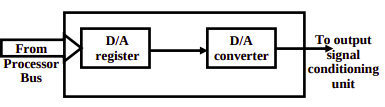
\includegraphics[width=0.6\textwidth]{images/output-interface.png}
    \caption{Output Interface (from CPU to an actuator)}
    \label{fig:output}
    \end{figure}
\end{itemize}

\section{Characteristics of Real-Time Systems}
We now discuss a few key characteristics of RTSs, which distinguish RTSs from non-RTSs. 
\begin{itemize}
    \item \textbf{Time constraints}: Every real-time task is associated with some time constraints. Though there are several timing constraints like \emph{deadline}, \emph{delay}, \emph{duration}, etc.; we will discuss the \emph{deadline} constraint here. A task \emph{deadline} specifies the time before which the task must complete and produce the results. Therefore, the onus is on the RTS to ensure that all tasks meet their respective time constraints. 
    \item \textbf{Correctness Criterion}: In traditional systems, the notion of correctness only refers to the logical correctness of the results. However, in RTSs, correctness implies not only logical correctness of the results, but also the time at which the results are produced is of utmost importance. A logically correct result produced after the deadline would be considered as an incorrect result. 
    \item \textbf{Concurrency}: An RTS usually needs to respond to several independent events within very short and strict time bounds. For instance, let us consider the chemical plant control discussed in section 2.1.1, which monitors the progress of a chemical reaction and controls the rate of reaction by changing the different parameters of reaction such as pressure, temperature, etc. These parameters are sensed using sensors fixed in the chemical reaction chamber. These sensors may generate data asynchronously at different rates. Therefore, the RTS must process data from all the sensors concurrently, otherwise signals may be lost which may lead into the malfunctioning of the system.
    \item \textbf{Custom Hardware}: An RTS is often implemented on custom hardware that is specifically designed and developed for the purpose at hand. For example, a cell phone utilizes processors which are tiny, supporting only those processing capabilities that are really necessary for cell phone operation. Additionally, these processors are designed to be power-efficient to conserve battery life. Another example is the embedded processor which is deployed in an Multi-Point Fuel Injection (MPFI) car. In this case, the processor is a 16 or 32-bit processor running at approximately 40 MHz. However, unlike the conventional PCs, a processor used in these car engines do not deal with processing chores such as screen-savers or a slew of different applications running simultaneously.
    \item \textbf{Reactive}: RTSs are often reactive. A reactive system is one in which an ongoing interaction between the computer and the environment is maintained. Traditional systems compute functions on the input data to generate the output data, as given in figure \ref{fig:trad-reac}.
    \begin{figure}[h]
    \centering
    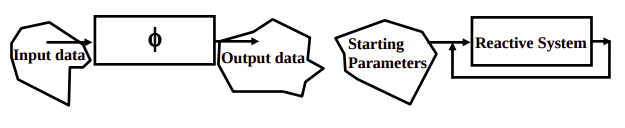
\includegraphics[width=0.8\textwidth]{images/trad-vs-reac.png}
    \caption{Traditional (left) versus Reactive (right) Systems}
    \label{fig:trad-reac}
    \end{figure}
    
    In contrast to traditional systems, RTSs don't generate any output data but enter into an ongoing interaction with their environment. In each interaction step, the results computed are used to carry out some actions on the environment. The reaction of the environment is sampled and is fed back to the system. We will get back to reactive systems again while discussing the library \texttt{StateGraph} \cite{stategraph}, which is used to model discrete event and reactive systems by hierarchical state machines in OpenModelica. 
    \item \textbf{Stability}: Under overload conditions, there are chances that the deadlines of non-critical tasks may not be fulfilled. Even though the RTSs need to continue to fulfil the deadlines of the most critical tasks. This is in contrast to the requirement of fairness for traditional systems under overload conditions. 
    \item \textbf{Exception Handling}: In this era of industrial automation, many RTSs work day-and-night and often operate without human operators. For example, let us consider a small automated chemical plant that is set up to work incessantly. When there are no human operators, it becomes increasingly difficult to take corrective actions on a failure. Even if no corrective actions can be immediate taken, it is desirable that a failure does not result in catastrophic situations. Ideally, a failure should be detected and the system should continue to operate in a gracefully degraded mode rather than shutting off abruptly. 
\end{itemize}

\section{Classification of Real-Time Systems}
Depending on the consequences of a task missing its deadline, a real-time task can be classified into three main types namely \textbf{Hard} real-time tasks, \textbf{Firm} real-time tasks, and \textbf{Soft} real-time tasks. 

\subsection{Hard Real-Time Tasks}
A hard real-time task is one that is constrained to produce its results within certain predefined time bounds. The system is considered to have failed whenever any of its hard real-time tasks does not produce its required results before the specified time bound. \\

An example of a system having hard real-time tasks is a robot. Let us consider that the robot cyclically carries out a number of activities including communication with the host system, logging all completed activities, sensing the environment to detect any obstacles present, tracking the objects of interest, path planning, etc. Now suppose that the robot suddenly encounters an obstacle. The robot must detect it and as soon as possible try to escape colliding with it. If it fails to respond to it quickly (i.e. the concerned tasks are not completed before the required time bound), then it would collide with the obstacle and the robot would be considered to have failed. Therefore detecting obstacles and reacting to it are hard real-time tasks, which must be completed within the confines of a stringent deadline. For hard real-time tasks in practical systems, the time bounds usually range from several microseconds to a few milliseconds. 

\subsection{Firm Real-Time Tasks}
Every firm real-time task is associated with some predefined deadline before which it is required to produce its results. However, unlike a hard real-time task, even when a firm real-time task does not complete within its deadline, the system is not considered to have failed. The late results are just discarded. In other words, the utility of the results computed by a firm real-time task becomes zero after the deadline. 

\begin{figure}[h]
\centering
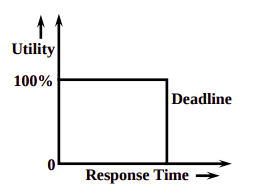
\includegraphics[width=0.4\textwidth]{images/firm-rts.png}
\caption{Utility of Result of a Firm Real-Time Task with Time}
\label{fig:firm-rts}
\end{figure}

The figure \ref{fig:firm-rts} shows the utility of the results produced by a firm real-time task as a function of time. For firm real-time tasks, the associated time bounds typically range from a few milliseconds to several hundreds of milliseconds.Firm real-time tasks typically proliferate in multimedia applications, such as video conferencing, where the delayed frames are simply discarded at the receiver-end. 

\subsection{Soft Real-Time Tasks}
Unlike hard and firm real-time tasks, the timing constraints on soft real-time tasks are not expressed as absolute values. Instead, the constraints are expressed either in terms of the average response times required.\\

Let us consider an example of handling request for seat reservation in railway reservation system. Once a request for a seat reservation is entered, the response should occur within 20 seconds on an average. The response may either be in the form of a printed ticket or a message on account of seats unavailability. Thus, we can set the constraint on the ticketing task as: At least in case of 95\% of reservation requests, the ticket should be processed and printed in less than 20 seconds. This is a soft real-time task where the timing costraints are expressed as average response time. 
\begin{figure}[h]
\centering
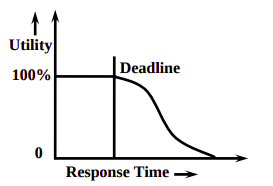
\includegraphics[width=0.4\textwidth]{images/soft-rts.png}
\caption{Utility of Result of a Soft Real-Time Task with Time}
\label{fig:soft-rts}
\end{figure}

Let us now analyze the impact of the failure of a soft real-time task to meet its deadline, by revisiting the example of the railway reservation system. If the ticket is printed within 20 seconds, we note that the system is working fine and experience the feeling of having instant results. In case of soft real-time tasks, missed deadlines do not result in system failures. However, the  utility of the results produced by a soft real-time task drops down continuously with time after the deadline expires,  as shown in figure \ref{fig:soft-rts}. For soft real-time tasks, the time bounds usually range from a fraction of a second to a few seconds. Now, we will summarize the major differences between hard and soft real-time tasks, as given in the table \ref{table:2}.  
\begin{table}[h]
\centering
\begin{tabular}{|c|c|c|}
 \hline
 \textbf{Characteristics} &  \textbf{Hard Real-Time} & \textbf{Soft Real-Time}\\
 \hline \hline
 Response time & Hard-required & Soft-desired\\ 
 \hline
 Peak load performance & Predictable & Degraded \\
 \hline
 Control of pace & Environment & Computer \\ 
 \hline
 Safety & Often critical & Non-critical \\
 \hline
 Size of data files & Small/medium & Large \\
 \hline
 Error detection & Autonomous & User assisted\\
 \hline
 Time bound & microseconds to few milliseconds & few seconds\\
 \hline
\end{tabular}
\caption{Comparison of Hard Real-Time Tasks and Soft Real-Time Tasks}
\label{table:2}
\end{table}

\chapter{Real-Time Task Scheduling}
For an RTS, we need to ensure that the system is capable of responding within a certain pre-specified time bound. These time bounds may vary depending upon the type of real-time task being handled. Thus, it calls for the requirement of a scheduler which would essentially determine the order in which the various tasks are to be taken up for execution by the operating system. Every operating system relies on one or more task schedulers to prepare the schedule of execution of various tasks. Each task scheduler is characterized by the scheduling algorithm it takes on. Here, we will discuss the available scheduling algorithms. 

\section{Types of Real-Time Task Scheduling Algorithms}
The two main types of schedulers are: clock-driven and event-driven. Furthermore, these two schedulers are classified into different subtypes, as given below:
\begin{enumerate}
    \setlength\itemsep{-0.2em}
    \item Clock-driven -- Table-driven and Cyclic
    \item Event-driven -- Simple priority based, Earliest Deadline First (EDF), and Rate Monotonic Analysis (RMA) 
\end{enumerate}

\subsection{Clock-Driven Scheduling}
Clock-driven schedulers make their scheduling decisions regarding which task to run next only at the clock interrupt points. For these schedulers, scheduling points are determined by timer interrupts. These schedulers are also known as off-line schedulers because these schedulers fix the schedule before the system starts to run. In order words, the scheduler predetermines the order of execution of tasks. Therefore, these schedulers incur very little run time overhead. However, a prominent shortcoming of this class of schedulers is that they can not satisfactorily handle aperiodic and sporadic (one that recurs at random instants) tasks since the exact time of occurrence of these tasks can not be predicted. For this reason, this type of schedulers is also known as static schedulers.  \\

There are two important clock-driven schedulers: table-driven and cyclic schedulers. Table-driven schedulers usually pre-compute which task would run when, and store this schedule in a table at the time the system is designed or configured. On the other hand, a cyclic scheduler repeats a pre-computed schedule. The pre-computed schedule needs to be stored only for one major cycle. 

\subsection{Event-Driven Scheduling}
In contrast to cyclic schedulers, event-driven schedulers can handle aperiodic and sporadic tasks more proficiently. However, event-driven schedulers are less efficient as they deploy more complex scheduling algorithms. Therefore, event-driven schedulers are less suitable for embedded applications as these are required to be of small size, low cost, and consume minimal amount of power. Next, we discuss the three important types of event-driven schedulers.\\

In foreground-background scheduler, which is possibly the simplest priority-driven preemptive scheduler, the real-time tasks in an application are run as fore-ground tasks. The sporadic, aperiodic, and non-real-time tasks are run as background tasks. Among the foreground tasks, at every scheduling point the highest priority task is taken up for scheduling. A background task can run when none of the foreground tasks is ready. In other words, the background tasks run at the least priority. \\

In EDF scheduling, the task having the shortest deadline is taken up for scheduling at every scheduling point. This scheduling technique has been proven to be an optimal uni-processor scheduling algorithm i.e., if a set of tasks cannot be scheduled under EDF, then no other scheduling algorithm can reasonably schedule this set of tasks.
\begin{table}[h]
\centering
\begin{tabular}{|c|c|c|}
 \hline
 \textbf{Parameter} &  \textbf{Clock-Driven Scheduling} & \textbf{Event-Driven Scheduling}\\
 \hline \hline
 Scheduling points & Timer interrupts & Events precluding clock interrupts\\ 
 \hline
 Design & Simple \& efficient & More sophisticated \\
 \hline
 Tasks & Periodic & Sporadic, aperiodic, and periodic \\
 \hline
 Applications & Embedded systems &  Moderate and
large-sized applications \\ 
 \hline
 Scheduling & Offline & Online \\
 \hline
\end{tabular}
\caption{Comparison of Clock-Driven Scheduling and Event-Driven Scheduling}
\label{table:3}
\end{table}

RMA, another important event-driven scheduling algorithm, assigns priorities to tasks based on their rates of occurrence. The lower the occurrence rate of a task, the lower is the priority assigned to it. A task having the highest occurrence rate (lowest period) is accorded the highest priority. Now, we will have a look at the comparison between clock-driven scheduling and event-driven scheduling, as shown in the table \ref{table:3} \cite{diff-clock-event}. 

\section{Dynamic Scheduling}
In a statically scheduled machine, the compiler determines the order of execution. On the other hand, in case of dynamic scheduling, the hardware determines which instructions to execute first. Here, we discuss some of the important dynamic scheduling algorithms. 

\subsection{Deferrable Scheduling with Least Actual Laxity First}
In real-time sensing and control systems, there is a need to monitor the Quality of Data (QoD) along with the Quality of Control (QoC). Keeping a track of QoD will let us know whether the sensor data has become stale. On the other hand, by following the QoC, we can check whether the deadline constraints of control transactions are fulfilled. There will always be a trade-off between maintaining the quality of real-time data objects and fulfilling the deadline constraints of control transactions while ensuring both QoD and QoC.\\

A dynamic scheduling algorithm named Deferrable Scheduling with Least Actual Laxity First (DS-LALF) is proposed in \cite{ds-lalf} to maintain the validity of real-time data objects. The actual laxity of a job is a measure of the spare time the job has before it misses its deadline -- by considering the time needed for higher priority jobs to be executed. In DS-LALF, control transactions are assigned lower priorities compared with the update transactions. Thus, it will maximize the QoD while affecting the schedulability of control transactions. \\     

An extension of the algorithm DS-LALF, named Co-LALF is presented to resolve the co-scheduling problem between update and control transactions in a real-time sensing and control system. The goal of Co-LALF is to construct a schedule that can meet the deadlines of all the periodic control transactions and can maximize the QoD as well. 

\subsection{Improving QoC using Flexible Timing Constraints}
As the closed-loop control systems are subject to perturbations, there is a need to design controllers to correct or limit the deviation caused by transient perturbations in the controlled system response. Though such controllers have been implemented using fixed timing constraints (sampling period and time delay), it prevents the controllers to execute dynamically, which in turn implies the wastage of resources when the system is in equilibrium along with quick reaction to perturbations. \\ 

A controller with flexible timing constraints is presented in \cite{qoc} which allows the design of discrete-time controllers depending upon a finite set of values for the sampling period and on a finite set of values for the time delay.  The flexible timing constraints for control tasks are defined in the form of a set of EXAST (EXAct start time Separation constrainT) values and a set of EXACT (EXAct start-to-Completion time-interval constrainT). The former refers to the set of sampling period values, whereas the latter refers to the set of time delays’ values.  The controller is designed with this assumption that the sampling will occur at (i.e., not after) EXAST and the actuation will complete at (i.e., not before) EXACT. \\

By selecting specific EXAST and EXACT values, the control task instance execution can be enabled to adapt according to the system dynamics. It means that when the controlled system response deviates due to perturbations, we will be able to speed up the execution of the controller in order to minimize such deviations, and when perturbations are not affecting the system, we can slow down the controller execution rate in order to save resources. 


\chapter{Concepts in Real-Time Operating Systems}
RTOSs are essentially responsible for ensuring that every real-time task meets its timing constraints requirements. An RTOS achieves this by using appropriate task scheduling techniques, which we have discussed in the previous chapter. Normally RTOSs provide flexibility to the programmers to select an appropriate scheduling policy. Therefore, deployment of an appropriate task scheduling technique out of the supported techniques is an important concern. In this chapter, we examine the important features that an RTOS is expected to support. We start by discussing the features of an RTOS followed by the issues that would arise if we attempt to use a GPOS such as UNIX or Windows for handling real-time applications. 

\section{Features of an RTOS}
We identify some important features indispensable to an RTOS, and especially those that are normally absent in a GPOS. 
\begin{itemize}
    \item \textbf{Clock and Timer Support}: Hard real-time application development often requires support of timer services with resolution of the order of a few microseconds. Moreover, some specific applications might require even finer resolution. As GPOS often does not provide time services with sufficiently high resolution, so we resort to RTOS for handling real-time tasks. 
    \item \textbf{Real-Time Priority Levels}: An RTOS must support static priority levels (also known as real-time priority levels). A priority level supported by an operating system is called static, when once the programmer assigns a priority value to a task, the operating system does not change it by itself. It may be noteworthy that all traditional operating systems dynamically change the priority levels of tasks to maximize system throughput. 
    \item \textbf{Fast Task Preemption}: For successful operation of a real-time application, whenever a high priority critical task arrives, an executing low priority task should provide the CPU to it instantly. The time duration for which a higher priority task waits before it is allowed to execute is quantitatively expressed as the corresponding task preemption time. Contemporary RTOS has task preemption times of the order of a few micro seconds. However, in a GPOS, the worst case task preemption time is usually of the order of a second. 
    \item \textbf{Predictable and Fast Interrupt Latency}: Interrupt latency is defined as the time delay between the appearance of an interrupt and the running of the corresponding interrupt service routine (ISR). In an RTOS, the upper bound on interrupt latency must be bounded and is expected to be less than a few micro seconds. This is especially important for hard real-time applications with timing requirements in microseconds or even less. 
\end{itemize}


\section{RTOS Fundamentals}
 Here, we present an introduction to real-time and multitasking concepts \cite{rtos-funda}, which are frequently used while using an RTOS.
 \begin{itemize}
     \item \textbf{Multitasking}: Each executing program is a task being controlled by the operating system. If an operating system can execute multiple tasks, it is said to be multitasking. A conventional processor can only execute a single task at a time -- but by rapidly switching between tasks a multitasking operating system can make it appear as if each task is executing concurrently. This is depicted in the figure \ref{fig:multitasking} which shows the execution pattern of three tasks (Task 1, Task 2, and Task 3) with respect to time. The task names are color coded and written on the left hand side of the figure \ref{fig:multitasking}.
     \begin{figure}[h]
    \centering
    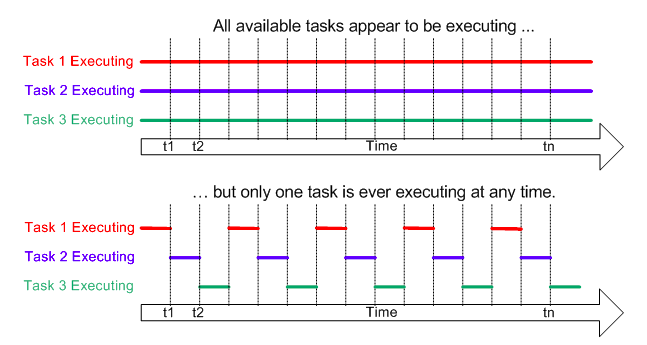
\includegraphics[width=0.82\textwidth]{images/multitasking.png}
    \caption{Multitasking Vs Concurrency}
    \label{fig:multitasking}
    \end{figure}
     \item \textbf{Scheduling}: The scheduler is the part of the kernel responsible for deciding which task should be executing at any particular time. The kernel can suspend and later resume a task many times during the task lifetime. The scheduling policy is the algorithm used by the scheduler to decide which task to execute at any point in time. The policy of a (non real-time) multi user system will most likely allow each task a ``fair” proportion of processor time. 
     \item \textbf{Context Switching}: As a task executes, it utilizes the processor/micro-controller registers and accesses RAM and ROM just as any other program. These resources together (the processor registers, stack, etc.) comprise the context of task execution. 
     
     A task is a sequential piece of code – it does not know when it is going to get suspended or resumed by the kernel and does not even know when this has happened. Consider the example of a task being suspended immediately before executing an instruction that sums the values contained within two processor registers. While the task is suspended other tasks will execute and may modify the processor register values. Upon resumption the task will not know that the processor registers have been altered – if it used the modified values the summation would result in an incorrect value. To prevent this type of error it is essential that upon resumption a task has a context identical to that immediately prior to its suspension. The operating system kernel is responsible for ensuring this and does so by saving the context of a task as it is suspended. When the task is resumed its saved context is restored by the operating system kernel prior to its execution. The process of saving the context of a task being suspended and restoring the context of a task being resumed is called context switching.
 \end{itemize}

Before discussing whether GPOS can be utilized for handling real-time tasks, we summarize the major differences between a GPOS and an RTOS \cite{rtos-guru}, as given in the table \ref{tab:gpos-rtos}. 
\begin{table}[h]
    \centering
    \begin{tabular}{|c|c|}
        \hline
        \textbf{GPOS} & \textbf{RTOS} \\
        \hline \hline
        Used for desktop PC and laptop. & Used for the embedded applications. \\
        \hline
        Process-based Scheduling &	Time-based scheduling \\
        \hline 
        Interrupt latency not important & Interrupt lag is minimal (in microseconds)\\
        \hline
        Kernel's operation may or may not be preempted &Kernel's operation can be preempted.\\
        \hline
    \end{tabular}
    \caption{Differences between a GPOS and an RTOS}
    \label{tab:gpos-rtos}
\end{table} 

 \section{Unix as an RTOS}
 Unix was originally developed for the mainframe computers. Since Unix and its variants are inexpensive and are now widely available, it is worthwhile to investigate whether Unix can be used in real-time applications. The traditional Unix operating system suffers from several shortcomings when used in real-time applications. A few of these shortcomings have been discussed below. 
 \begin{itemize}
     \item \textbf{Non-Preemptive Kernel}: One of the biggest problems that real-time programmers face while using Unix for real-time application development is that Unix kernel cannot be preempted. That is, all interrupts are disabled when any operating system routine runs. 
     
     A process running in kernel mode cannot be preempted by other processes. In other words, the Unix kernel is non-preemptive. On the other hand, the Unix system does preempt processes running in the user mode. As a consequence, even when a low priority process makes a system call, the high priority processes would have to wait until the system call completes. The longest system calls may take up to several hundreds of milliseconds to complete. 
     \item \textbf{Dynamic Priority Levels}: In Unix systems, real-time tasks can not be assigned static priority values. This is due to the fact that the operating system alters the priority value, after a programmer sets it. This makes it very difficult to schedule real-time tasks using algorithms such as RMA or EDF, since both these schedulers assume that once task priorities are assigned, it should not be altered by any other parts of the operating system. 
 \end{itemize}
 
\section{Windows as an RTOS}
Microsoft’s Windows operating systems have evolved over the years from the naive DOS (Disk Operating System). As several new versions of Windows kept on appearing by way of upgrades, the Windows code was completely rewritten in 1998 to develop the Windows NT system. Since the code was completely rewritten, Windows NT system was much more stable than the earlier DOS-based systems. The later versions of Microsoft’s operating systems were descendants of the Windows NT. Here, we consider only the Windows NT and its descendants.\\

Windows NT has several features which are very desirable for real-time applications such as support for multi-threading, real-time priority levels, and timer. Moreover, the clock resolutions are sufficiently fine for most real-time applications. Windows NT supports 32 priority levels. Each process belongs to one of the following priority classes: idle, normal, high, real-time. By default, the priority class at which an application runs is normal. NT uses priority-driven pre-emptive scheduling and threads of real-time priorities have precedence over all other threads including kernel threads. \\

In spite of the impressive support that Windows provides for real-time program development as discussed above, it is neither advisable nor feasible to use NT for hard real-time applications, for example, at the controller level with sub-millisecond precision as pointed  out in \cite{windowsnt-k}. NT may still be useful for applications that can tolerate occasional deadline misses, and have delay/response time requirements in the tens to hundreds of milliseconds range. At the end, we present a comparison of the extent to which some of the basic features required for real-time programming are provided by Windows NT and Unix, as given in the table \ref{table:4}. 
\begin{table}[h]
\centering
\begin{tabular}{|c|c|c|}
 \hline
 \textbf{Real-Time Features} &  \textbf{Windows NT} & \textbf{Unix}\\
 \hline \hline
 DPCs & Yes & No \\
 \hline
 Real-Time priorities & Yes & No \\
 \hline
 Locking virtual memory & Yes & Yes\\
 \hline 
 Timer precision & 1 msec & 10 msec \\
 \hline
 Asynchronous I/O & Yes & No\\
 \hline
\end{tabular}
\caption{Windows NT versus Unix}
\label{table:4}
\end{table}



\chapter{Tools for enabling Real-Time Features}
In this chapter, we will explain some of the open-source tools which are being utilized to enable real-time constraints across various platforms like an operating system, open-source software like Scilab \cite{scilab}, OpenModelica \cite{OM},  and micro-controllers like Arduino \cite{arduino}. \\

We will begin our discussion with POSIX, which stands for Portable Operating System Interface. ``X" has been suffixed to the  abbreviation to make it sound Unix-like. Over the last decade, POSIX has become an important standard in the operating systems area including real-time operating systems. The importance of  POSIX can be evaluated from the fact that nowadays it is rare to come across a commercial operating system that is not POSIX-compliant. POSIX started as an open software initiative.

\section{Linux as a Real-Time System}
Here, we discuss some of the important patches or extension like PREEMPT\_RT, RTLinux, RTAI, etc. which make Linux into a real-time system. 
\subsection{PREEMPT\_RT}
The PREEMPT\_RT patch (aka the -rt patch or RT patch) makes Linux into a real-time system \cite{rtlinux}. If our embedded device has some ``must have" deadlines to respond to then the PREEMPT\_RT patch would probably be sufficient. What PREEMPT\_RT gives us over the normal kernel is not only faster response times, but more importantly, it removes all unbounded latency. An unbounded latency is where the amount of delay that can occur is dependent on the situation. For example, let us consider the case of unfair reader writer locks, where the writer has to wait for there to be no readers before it can take the lock. Because new readers can continually take the lock at any time while the writer is waiting, the writer may never get the lock. This is a prime example of an unbounded latency on the writer.\\

According to Mr. Rostedt, PREEMPT\_RT is really good enough for robotics, stock exchanges, and for computers that have to interface with the ``Hard" real-time software.

\begin{figure}[h]
\centering
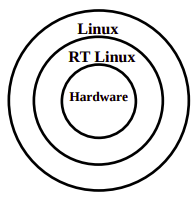
\includegraphics[width=0.3\textwidth]{images/rtlinux.png}
\caption{Structure of RTLinux}
\label{fig:rt-linux}
\end{figure}

\subsection{Real-Time Linux (RTLinux)}
RTLinux runs along with a Linux system \cite{embd-rtlinux}. The real-time kernel sits between the hardware and the Linux system, as shown in the figure \ref{fig:rt-linux}. The RT kernel intercepts all interrupts generated by the hardware. If an interrupt is to cause a real-time task to run, the real-time kernel preempts Linux, if Linux is running at that time, and lets the real-time task run. Thus, in effect Linux runs as a task of RTLinux. \\

The real-time applications are written as loadable kernel modules. In essence, real-time applications run in the kernel space. In the RTLinux approach, there are effectively two independent kernels: real-time kernel and Linux kernel. Therefore, this approach is also known as the dual-kernel approach as the real-time kernel is implemented outside the Linux kernel. Any task that requires deterministic scheduling is run as a real-time task. These tasks preempt Linux whenever they need to execute and yield the CPU to Linux only when no real-time task is ready to run.\\ 

Compared to the micro-kernel approach, the following are the shortcomings of the dual-kernel approach.
\begin{itemize}
    \item \textbf{Duplicated Coding Efforts}: Tasks running in the real-time kernel can not make full use of the Linux system services such as file systems, networking, and so on. In fact, if a real-time task invokes a Linux service, it will be subject to the same preemption problems that prohibit Linux processes from behaving in a deterministic fashion. As a result, new drivers and system services must be created specifically for the real-time kernel – even when equivalent services already exist for Linux.
    \item \textbf{Fragile Execution Environment}: Tasks running in the real-time kernel do not benefit from the memory management unit (MMU)-protected environment that Linux provides to the regular non-real-time processes. Instead, they run unprotected in the kernel space. Consequently, any real-time task that contains a coding error such as a corrupt C pointer can easily cause a fatal kernel fault. This is serious problem since many embedded applications are safety-critical in nature.
    \item \textbf{Limited Portability}: In the dual-kernel approach, the real-time tasks are not Linux processes at all; but programs written using a small subset of POSIX APIs. To aggravate the matter, different implementations of dual-kernels use different APIs. As a result, real-time programs written using one vendor's RT-Linux version may not run on another vendor.
    \item \textbf{Programming Difficulty}: RTLinux kernels support only a limited subset of POSIX APIs. Therefore, application development takes more effort and time. 
\end{itemize}

\subsection{Real-Time Application Interface (RTAI) for Linux}
RTAI (\url{https://www.rtai.org/}) is a real-time extension for the Linux kernel, which lets users write applications with strict timing constraints for Linux \cite{wiki-rtai} \cite{real-time-cap}. It provides deterministic response to interrupts, POSIX-compliant and native RTAI real-time tasks. RTAI supports several architectures, including x86-64, and ARM.\\

RTAI consists mainly of two parts: an Adeos-based patch \cite{adeos} to the Linux kernel which introduces a hardware abstraction layer, and a broad variety of services which make lives of real-time programmers easier. This way, RTAI can transparently take over interrupts while leaving the processing of all others to Linux. \\

\subsection{Subtle Differences between RTAI and RTLinux}
Here, we investigate the subtle differences while using RTAI vis-\`a-vis RTLinux in real-time implementations. Prof. Paolo Mantegazza started the RTAI project based on Victor Yodaiken's RTLinux v. 1 \cite{embd-rtlinux}. Since then, RTLinux and RTAI have gone through long development paths on their own. Despite the fact that they're not API-compatible, their functionalities are very similar \cite{rtai-linux-journal}. All key primitives and services exist in both packages. Both offer:
\begin{itemize}
    \setlength\itemsep{-0.2em}
    \item A small real-time core
    \item One-shot and periodic timer support
    \item Real-time scheduler
    \item Real-time threads
    \item Real-time FIFOs and shared memory
    \item Real-time interrupt handler
\end{itemize}

To summarize, RTAI provides a more practical API while RTLinux is more elegant. On the other hand, RTAI is more elegant in how it integrates into the Linux kernel. The RTAI team makes a constant effort to add features that people ask for, and thus its API has grown to become reasonably extensive. For example, RTAI includes clock (8254 and APIC) calibration, dynamic memory management for realtime tasks, LXRT (Linux Extension for Real-Time) to bring soft/hard real-time capabilities into user space, remote procedure calls, and mailboxes. Due to the practicality of RTAI API,  an open source project named  RTAI-Lab aims to provide a common structure framework for the integration of RTAI into the Scilab environment \cite{scilab-rtai}. With RTAI-Lab and Scilab, it is possible to obtain a complete open source environment for designing control systems and test them in real physical systems as demonstrated in \cite{scilab-rtai}. This software tool-chain (RTAI-Lab and Scilab) is equivalent to the proprietary software for control systems Labview or Dspace.\\ 

The RTLinux team aims to keep their real-time Linux extensions as predictable as possible, adding only features that won't hurt designs and compatibility in the future. In short, the RTLinux API is more consistent, but many practitioners prefer to use RTAI.  

\section{OpenModelica for Real-Time Systems}
OpenModelica \cite{OM} is an open-source Modelica-based modeling and simulation environment intended for industrial and academic usage. The goal with the OpenModelica effort is to create a comprehensive Open Source Modelica modeling, compilation and simulation environment based on free software distributed in binary and source code form for research, teaching, and industrial usage. In this section, we present two tools available in OpenModelica -- Modelica.\texttt{StateGraph} and Real-Time simulation flag -- which can be used to characterize reactive systems and the physical time concept of real-time systems. 

\subsection{Modelica.StateGraph}
Modelica is primarily a modeling language that allows specification of mathematical models of complex natural or man-made systems, e.g., for the purpose of computer simulation of dynamic systems
where behavior evolves as a function of time \cite{OMbook}. Modelica is also an object-oriented, equation-based programming language, oriented toward computational applications with high complexity requiring high performance.

\begin{figure}[h]
\centering
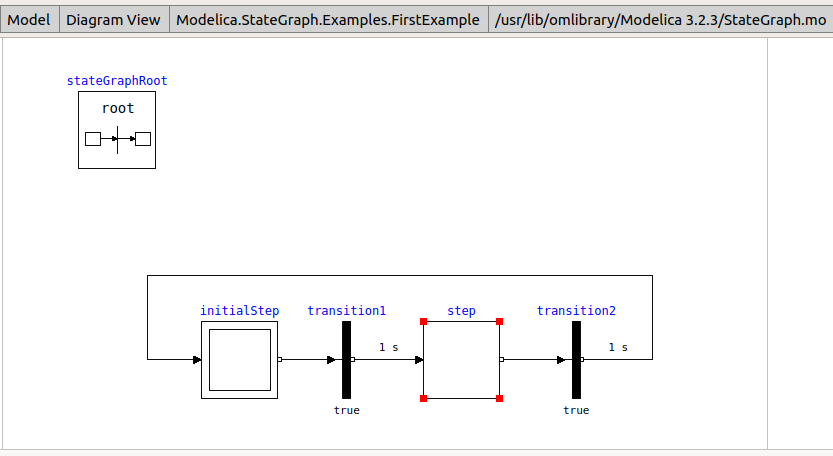
\includegraphics[width=0.88\textwidth]{images/stategraph.png}
\caption{Basic Example of \texttt{StateGraph} in OpenModelica}
\label{fig:stategraph}
\end{figure}

Modelica modeling formalism matches all the requirements for characterizing reactive systems, as discussed in section 2.3. For instance, concurrency is natural since modeled objects evolve concurrently over time. Time aspects can be efficiently modeled, and specified behavior is deterministic. Since Modelica is a declarative formalism, models should hopefully be somewhat amenable to formal verification techniques for enhancing reliability. Modeled subsystems can be realized as efficient implementations of reactive computer systems that interact directly with the physical environment in real-time. Alternatively, both the reactive system and the surrounding physical environment can be modeled and simulated. A third alternative is to mix simulated subsystems with hardware components, that is, hardware-in-the-loop simulation \cite{hil}.\\ 

Library \texttt{StateGraph} is a free Modelica package providing components to model discrete event and reactive systems in a convenient way \cite{stategraph}. It is based on the JGrafchart method and takes advantage of Modelica features for the ``action" language. JGrafchart is a further development of Grafcet to include elements of StateCharts that are not present in Grafcet/Sequential Function Charts. Therefore, the \texttt{StateGraph} library has a similar modeling power as StateCharts but avoids some deficiencies of StateCharts. \\

A basic example of \texttt{StateGraph} is shown in the figure \ref{fig:stategraph}. In JGrafcharts, Grafcet, Sequential Function Charts and StateCharts, actions are formulated within a step. Such actions are distinguished as entry, normal, exit and abort actions. For example, a valve might be opened by an entry action of a step and might be closed by an exit action of the same step. In \texttt{StateGraph}, this is not possible due to Modelica's ``single assignment rule" that requires that every variable is defined by exactly one equation. For example, via the ``SetBoolean" component, the valve variable is set to true when the \texttt{StateGraph} is in particular steps. \\ 

This feature of a \texttt{StateGraph} is very useful, since it allows a Modelica translator to guarantee that a given \texttt{StateGraph} has always deterministic behaviour without conflicts. In the other methodologies this is much more cumbersome. For example, if two steps are executed in parallel and both step actions modify the same variable, the result is either non-deterministic or non-obvious rules have to be defined which action takes priority. In a \texttt{StateGraph}, such a situation is detected by the translator resulting in an error, since there are two equations to compute one variable. \\

\subsection{Simulation Flags in OpenModelica}
Apart from \texttt{StateGraph} library, we can use a simulation flag \cite{flags} for real-time synchronization in OpenModelica . This flag can be enabled by using \texttt{-rt=value} or \texttt{-rt value}. The value specifies the scaling factor for real-time synchronization (0 disables). A value greater than 1 means the simulation takes a longer time to simulate. 
\begin{figure}[h]
\centering
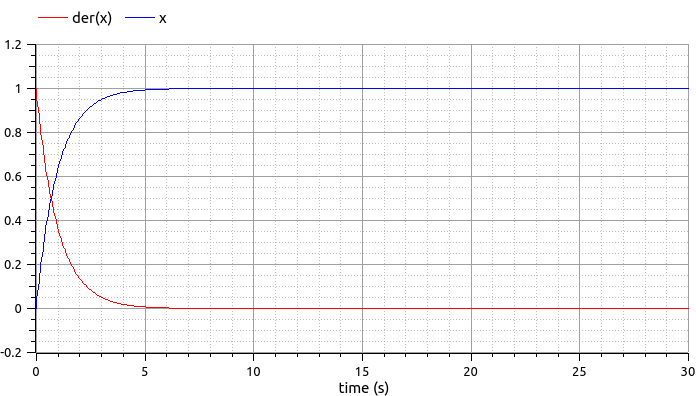
\includegraphics[width=0.8\textwidth]{images/flag.png}
\caption{Simulation of a First-Order System in OpenModelica}
\label{fig:first-order-rt}
\end{figure}
For our study, we simulated a first order model by enabling the real-time flag. It was observed that with flag enabled, the simulation takes physical time into consideration, as discussed in second chapter. Thus, the real-time simulation runs for the exact duration of the simulation. The output of the simulation is as shown in the figure \ref{fig:first-order-rt} and the video of the simulation is available on \href{https://youtu.be/s2oELiNWK40}{YouTube}.


\section{FreeRTOS Task Implementation in Arduino IDE}
FreeRTOS is a class of RTOS for embedded devices which is small enough to be run on 8/16-bit micro-controllers, although its use is not limited to these micro-controllers \cite{freertos}. It is open-source and it's code is available on GitHub (\url{https://github.com/FreeRTOS}).\\

As FreeRTOS can run on 8-bit MCU so it can also be run on Arduino Uno board. We have to just download the FreeRTOS library and then start implementing the code using APIs. We will consider an example of blinking two LEDs at different rates on an Arduino Uno using FreeRTOS. For this example, we will consider the following tasks:
\begin{itemize}
    \setlength\itemsep{-0.2em}
    \item LED blink at Digital pin 8 with 200ms frequency.
    \item LED blink at Digital pin 7 with 300ms frequency.
    \item Print numbers in serial monitor with 500ms frequency. 
\end{itemize}

According to the FreeRTOS structure, we will include the Arduino FreeRTOS header file. Then we need to make function prototypes. As we have three tasks, so we will make three functions and it's prototypes, as given below:
\begin{verbatim}
    #include <Arduino_FreeRTOS.h>
    void TaskBlink1(void *pvParameters);
    void TaskBlink2(void *pvParameters);
    void Taskprint(void *pvParameters);
\end{verbatim}

In \texttt{void setup()} function, we will initialize serial communication at 9600 bits per second and create all three tasks using \texttt{xTaskCreate()} API of FreeRTOS. Initially, we will make the priorities of all tasks as ‘1’ and start the scheduler.
\begin{verbatim}
    void setup() {
    Serial.begin(9600);
    xTaskCreate(TaskBlink1, "Task1", 128, NULL, 1, NULL);
    xTaskCreate(TaskBlink2, "Task2 ", 128, NULL, 1, NULL);
    xTaskCreate(Taskprint, "Task3", 128, NULL, 1, NULL);   
    vTaskStartScheduler();
}
\end{verbatim}

Now, we will implement the required functions as shown below for the first task i.e., LED blink at Digital pin 8 with 200ms frequency. 
\begin{verbatim}
    void TaskBlink1(void *pvParameters) {
    pinMode(8, OUTPUT);
    while(1){
        digitalWrite(8, HIGH);   
        vTaskDelay( 200 / portTICK_PERIOD_MS ); 
        digitalWrite(8, LOW);    
        vTaskDelay( 200 / portTICK_PERIOD_MS ); 
    	}
    }
\end{verbatim}

Similarly, we can implement second task i.e., LED blink at Digital pin 7 with 300ms frequency. The third task i.e., Print numbers in serial monitor with 500ms frequency will be written as
\begin{verbatim}
    void Taskprint(void *pvParameters)  {
    int counter = 0;
    while(1){
        counter++;
        Serial.println(counter);
        vTaskDelay( 500 / portTICK_PERIOD_MS ); 
    	}
    }
\end{verbatim}

Thus, we can now run this code on Arduino Uno to perform three tasks as mentioned above. The code to run these tasks using FreeRTOS is available in a \href{https://github.com/SudhakarKuma/MTech_Seminar_June_2020/tree/master/FreeRTOS_Arduino_codes}{GitHub repository}. 

\begin{figure}[h]
\centering
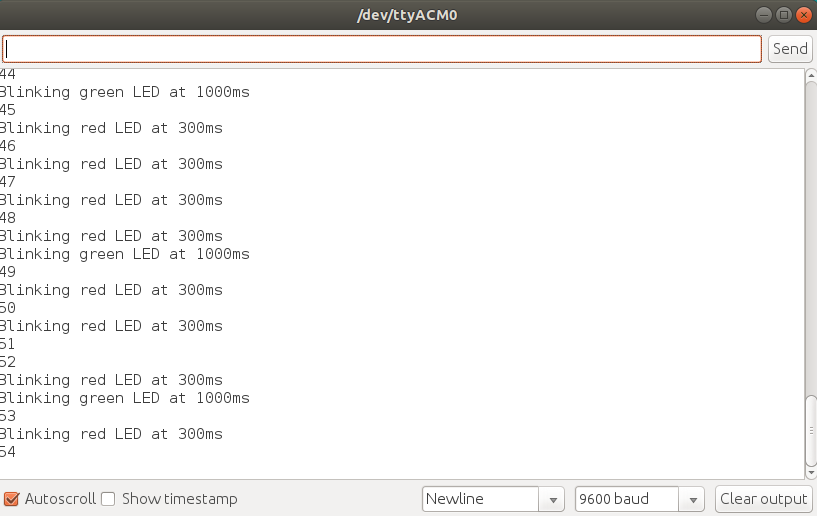
\includegraphics[width=0.75\textwidth]{images/Arduino-ide-tasks.png}
\caption{Serial Monitor of Arduino IDE with the Tasks (being executed)}
\label{fig:arduino-leds-serial-mon}
\end{figure}


The simulation results on the serial monitor of Arduino IDE is as shown in the figure \ref{fig:arduino-leds-serial-mon} and the video of the simulation is available on \href{https://youtu.be/SBuHO7kwZ0Y}{YouTube}. In this video, the red LED and the green LED are blinking with 300ms frequency and 1000ms frequency, respectively. This significant difference in the two frequencies facilitates the clear visualization of two LEDs blinking at different rates.  


\section{RTOS versus Bare-Metal Scheduling}
The use of an RTOS or a bare-metal scheduler is a popular topic of debate among embedded system developers. The supporters of bare metal argue that they can use a combination of priority-based interrupts and timers to get RTOS-equivalent behavior with better performance and memory footprint. The RTOS side stresses ease of scheduling and system integration, for starters. We will discuss some of the important reasons why a developer may decide to start with an RTOS over a bare-metal scheduler \cite{rtos-need}. 

\begin{itemize}
    \item \textbf{Concurrency}: Micro-controller based systems typically only have a single processing core but there is always a need to execute multiple tasks. In applications where tasks need to appear to be executing at the same time or concurrently, the use of an RTOS makes sense. An RTOS can have multiple tasks simultaneously in memory and can switch between them based on events and priorities. A bare-metal scheduler could be used, but tasks in a bare-metal system usually execute one at a time and not concurrently.
    \item \textbf{Pre-emption}: Pre-emption is the ability of an operating system to temporarily suspend a task in order to execute a higher-priority task. If the embedded software that is being developed requires the need to prioritize tasks and interrupt tasks that are currently running, an RTOS is the go-to operating system. The nature of most RTOS systems is to determine which tasks should be executing at any given time based on the priority of the task and system conditions. A bare-metal scheduler can be developed that emulates this type of behavior using priority-based interrupts, but the use of an RTOS is more appropriate for the situation.
    \item \textbf{Available RAM}: The amount of available RAM on a micro-controller can be a decisive factor as to whether an RTOS or a bare-metal scheduler should be used. Resource-constrained systems that have less than 4 kilobytes of RAM can be difficult to fit within memory due to the fact that each task has its own task control block and stack. A bare-metal system, on the other hand, typically has just the one stack and doesn't require the extra overhead necessary to keep track of the state of each system task. At a minimum, micro-controller-based systems should have at least 4 kilobytes of RAM (preferably 8 kB) before going with an RTOS solution.
    \item \textbf{Available Flash}: Since a developer should look at how much RAM is available on a system before deciding to go with a RTOS, he or she should also look at how much flash space is available. RTOS systems don't take up much flash space, usually on the order of eight to 10 kB, but if the micro-controller only has 16 kB of flash space, there really isn't much room left for the application code. If the micro-controller has at least 32 kB of flash space, then the system is a good candidate for the use of an RTOS. Anything less and it might be time to dust off the bare-metal scheduler or upgrade the hardware.
    \item \textbf{Synchronization Tools}: One of the problems with using a bare-metal scheduler is that it lacks synchronization tools that are included by default in a RTOS. For example, an RTOS has Mutexes that can be used to protect a shared resource, and Semaphores that can be used to signal and synchronize tasks and message queues to transfer data between tasks. Properly designing and implementing these core software features isn't trivial, and adding them into a bare-metal scheduler from scratch will undoubtedly inject bugs. If a system has multiple tasks and protected resources that require synchronization, then the use of an RTOS is the wise decision.
    \item \textbf{Third-Party Software}: One of the problems facing many developers today is how to integrate third-party software stacks and tools into their embedded system. Few developers want to write a TCP/IP or USB stack. Many of the third-party stacks and tools that are available on the market are compatible with various RTOSs. The use of an RTOS makes these components plug-and-play within the software and can drastically accelerate software development. The decision to use third-party software could be a major indicator that an RTOS should be used over a bare-metal scheduler.
    \item \textbf{Ease of Use}: RTOS systems are readily available for nearly every micro-controller and for nearly application imaginable. Whether a developer just wants to create a rapid prototype or build a robust safety-critical system, an RTOS exists that developers can leverage and get up and running fairly quickly. Creating tasks and utilizing RTOS tools is easy and very powerful, but developers need to beware that they properly analyze their tasks and think through their system design. An RTOS is a powerful tool, but improper use can result in tragic results.
\end{itemize}

\chapter{Conclusion}
In this report, we discussed the difference between a real-time task and a non-real-time task. We realised that a  non-real-time task is not associated with any time bounds.  A few examples of non-real-time tasks  are:  batch  processing  jobs,  e-mail,  and  back  ground  tasks  such  as  event  loggers.   One may however argue that even these tasks, in the strict sense of the term, do have certain time bounds.  For example, an e-mail is expected to reach its destination at least within a couple of hours of being sent.  Similar is the case with a batch processing job such as pay-slip printing. What then really is the difference between a non-real-time task and a soft real-time task?  For non-real-time  tasks,  the  associated  time  bounds  are  typically  of  the  order  of  a  few  minutes, hours or even days.  In contrast, the time bounds associated with soft real-time tasks are at most of the order of a few seconds. \\ 

Along with this, we compared the functions of an RTOS and a GPOS. Next, we also discussed the various scheduling techniques which should be exploited to deal with real-time sensing and control systems. At the end, we investigated the available real-time control methodologies using open-source tools like RTLinux, RTAI-Lab, \texttt{StateGraph}, FreeRTOS, etc. We also ran a few simulations on OpenModelica and Arduino. It was found that these open-source tools perform well while handling real-time control. However, there is a need to run the simulations on complex systems to check whether the real-time tools discussed are able to meet the hard real-time constraints. 

\begin{thebibliography}{111}
%\bibitem{framevspc}
%Mainframe vs PC, \url{https://blog.syncsort.com/2018/10/mainframe/mainframes-vs-pc-4-things/}

\bibitem{NPTEL}
Introduction to Real-Time Systems, \url{https://nptel.ac.in/content/storage2/courses/108105057/Pdf/Lesson-28.pdf}

\bibitem{rts}
Real-Time Systems, \url{https://users.ece.cmu.edu/~koopman/des_s99/real_time/}

\bibitem{unsw}
Real-Time Systems, \url{https://www.cse.unsw.edu.au/~cs9242/08/lectures/09-realtimex2.pdf}

\bibitem{rtlinux}
Intro to Real-Time Linux for Embedded Developers, \url{https://www.linuxfoundation.org/blog/2013/03/intro-to-real-time-linux-for-embedded-developers/}

\bibitem{stategraph}
Modelica.StateGraph, \url{https://build.openmodelica.org/Documentation/Modelica.StateGraph.html}

\bibitem{diff-clock-event}
Difference between Clock-driven and Event-driven Scheduling, \url{https://www.geeksforgeeks.org/difference-between-clock-driven-and-event-driven-scheduling/}

\bibitem{roundrobin}
Program for Round Robin scheduling, \url{https://www.geeksforgeeks.org/program-round-robin-scheduling-set-1/}

\bibitem{ds-lalf}
S. Han, K. Lam, J. Wang, K. Ramamritham and A. K. Mok, "On Co-Scheduling of Update and Control Transactions in Real-Time Sensing and Control Systems: Algorithms, Analysis, and Performance," in IEEE Transactions on Knowledge and Data Engineering, vol. 25, no. 10, pp. 2325-2342, Oct. 2013, doi: 10.1109/TKDE.2012.173.

\bibitem{qoc}
P. Marti, J. M. Fuertes, G. Fohler and K. Ramamritham, "Improving quality-of-control using flexible timing constraints: metric and scheduling," 23rd IEEE Real-Time Systems Symposium, 2002. RTSS 2002., Austin, Texas, USA, 2002, pp. 91-100, doi: 10.1109/REAL.2002.1181565.

\bibitem{rtos-funda}
RTOS Fundamentals, \url{https://www.freertos.org/implementation/a00002.html}

\bibitem{windowsnt-k}
Ramamritham, K. (1999, December). Can real-time systems be built from off-the-shelf components?. In Proceedings Sixth International Conference on Real-Time Computing Systems and Applications. RTCSA'99 (Cat. No. PR00306) (pp. 226-226). IEEE.

\bibitem{rtos-guru}
Real-time operating system (RTOS): Components, Types, Examples, \url{https://www.guru99.com/real-time-operating-system.html}

\bibitem{scilab}
Scilab, Open source software for numerical computation, \url{https://www.scilab.org/}

\bibitem{OM}
OpenModelica, Open-source Modelica-based modeling and simulation environment intended for industrial and academic usage, \url{https://openmodelica.org/}

\bibitem{arduino}
Arduino, Open-source electronics platform based on easy-to-use hardware and software, \url{https://www.arduino.cc/}

\bibitem{embd-rtlinux}
Real-Time Linux, \url{https://www.embedded.com/real-time-linux/}

\bibitem{wiki-rtai}
RTAI - Wikipedia, \url{https://en.wikipedia.org/wiki/RTAI} 

\bibitem{real-time-cap}
Arm, J., Bradac, Z., \& Kaczmarczyk, V. (2016). Real-time capabilities of Linux RTAI. IFAC-PapersOnLine, 49(25), 401-406.

\bibitem{adeos}
Adaptive Domain Environment for Operating Systems - Wikipedia \url{https://en.wikipedia.org/wiki/Adaptive_Domain_Environment_for_Operating_Systems}

\bibitem{rtai-linux-journal}
RTAI: Real-Time Application Interface, \url{https://www.linuxjournal.com/article/3838}

\bibitem{scilab-rtai}
C. Meza, J. A. Andrade-Romero, R. Bucher and S. Balemi, "Free open source software in control engineering education: A case study in the analysis and control design of a rotary inverted pendulum," 2009 IEEE Conference on Emerging Technologies \& Factory Automation, Mallorca, 2009, pp. 1-8, doi: 10.1109/ETFA.2009.5347162.

\bibitem{OMbook}
Peter Fritzson, Principles of Object-Oriented Modeling and Simulation with Modelica 3.3: A Cyber-Physical Approach, ISBN: 978-1-118-85912-4, April 2015, Wiley-IEEE Press. 

\bibitem{hil} 
Hardware-in-the-loop simulation - Wikipedia, \url{https://en.wikipedia.org/wiki/Hardware-in-the-loop_simulation}

\bibitem{flags}
OpenModelica (C-runtime) Simulation Flags, \url{https://www.openmodelica.org/doc/OpenModelicaUsersGuide/latest/simulationflags.html}

\bibitem{freertos}
Arduino FreeRTOS Tutorial,\\
\url{https://circuitdigest.com/microcontroller-projects/arduino-freertos-tutorial1-creating-freertos-task-to-blink-led-in-arduino-uno}

\bibitem{rtos-need}
Do You Need an RTOS?, \url{https://www.designnews.com/electronics-test/do-you-need-rtos-yes-and-here-are-7-reasons-why/29593780546421}
\end{thebibliography}

\end{document}

